\documentclass{article}

\usepackage{fancyhdr}
\usepackage{extramarks}
\usepackage{amsmath}
\usepackage{amsthm}
\usepackage{amsfonts}
\usepackage{tikz}
\usepackage[plain]{algorithm}
\usepackage{algpseudocode}
\usepackage{listings} 
\usepackage{neuralnetwork}
\usetikzlibrary{automata,positioning}

\usepackage{color}

\definecolor{dkgreen}{rgb}{0,0.6,0}
\definecolor{gray}{rgb}{0.5,0.5,0.5}
\definecolor{mauve}{rgb}{0.58,0,0.82}

\lstset{frame=tb,
  language=Python,
  aboveskip=3mm,
  belowskip=3mm,
  showstringspaces=false,
  columns=flexible,
  basicstyle={\small\ttfamily},
  numbers=none,
  numberstyle=\tiny\color{gray},
  keywordstyle=\color{blue},
  commentstyle=\color{dkgreen},
  stringstyle=\color{mauve},
  breaklines=true,
  breakatwhitespace=true,
  tabsize=3
}
%
% Basic Document Settings
%

\topmargin=-0.45in
\evensidemargin=0in
\oddsidemargin=0in
\textwidth=6.5in
\textheight=9.0in
\headsep=0.25in

\linespread{1.1}

\pagestyle{fancy}
\lhead{\hmwkAuthorName}
\chead{\hmwkClass\: \hmwkTitle}
\rhead{\firstxmark}
\lfoot{\lastxmark}
\cfoot{\thepage}

\renewcommand\headrulewidth{0.4pt}
\renewcommand\footrulewidth{0.4pt}

\setlength\parindent{0pt}

%
% Create Problem Sections
%

\newcommand{\enterProblemHeader}[1]{
    \nobreak\extramarks{}{Task \arabic{#1} continued on next page\ldots}\nobreak{}
    \nobreak\extramarks{Task \arabic{#1} (continued)}{Problem \arabic{#1} continued on next page\ldots}\nobreak{}
}

\newcommand{\exitProblemHeader}[1]{
    \nobreak\extramarks{Task \arabic{#1} (continued)}{Problem \arabic{#1} continued on next page\ldots}\nobreak{}
    \stepcounter{#1}
    \nobreak\extramarks{Task \arabic{#1}}{}\nobreak{}
}

\setcounter{secnumdepth}{0}
\newcounter{partCounter}
\newcounter{homeworkProblemCounter}
\setcounter{homeworkProblemCounter}{1}
\nobreak\extramarks{Task \arabic{homeworkProblemCounter}}{}\nobreak{}

%
% Homework Problem Environment
%
% This environment takes an optional argument. When given, it will adjust the
% problem counter. This is useful for when the problems given for your
% assignment aren't sequential. See the last 3 problems of this template for an
% example.
%
\newenvironment{homeworkProblem}[1][-1]{
    \ifnum#1>0
        \setcounter{homeworkProblemCounter}{#1}
    \fi
    \section{Task \arabic{homeworkProblemCounter}}
    \setcounter{partCounter}{1}
    \enterProblemHeader{homeworkProblemCounter}
}{
    \exitProblemHeader{homeworkProblemCounter}
}

%
% Homework Details
%   - Title
%   - Due date
%   - Class
%   - Section/Time
%   - Instructor
%   - Author
%

\newcommand{\hmwkTitle}{Lab\ \#1}
\newcommand{\hmwkDueDate}{September 25, 2019}
\newcommand{\hmwkClass}{CSCI964 Computational Intelligence}
\newcommand{\hmwkClassTime}{2.14}
\newcommand{\hmwkClassInstructor}{Zhifeng Wang}
\newcommand{\hmwkAuthorName}{\textbf{Mei Wangzhihui}}
\newcommand{\hmwkAuthorNum}{\textbf{2019124044}}
%
% Title Page
%

\title{
    \vspace{2in}
    \textmd{\textbf{\hmwkClass:\ \hmwkTitle}}\\
    % \normalsize\vspace{0.1in}\small{Due\ on\ \hmwkDueDate\ at 3:10pm}\\
    % \vspace{0.1in}\large{\textit{\hmwkClassInstructor\ \hmwkClassTime}}
    \vspace{3in}
}

\author{\hmwkAuthorName\ \hmwkAuthorNum}
\date{}

\renewcommand{\part}[1]{\textbf{\large Part \Alph{partCounter}}\stepcounter{partCounter}\\}

%
% Various Helper Commands
%

% Useful for algorithms
\newcommand{\alg}[1]{\textsc{\bfseries \footnotesize #1}}

% For derivatives
\newcommand{\deriv}[1]{\frac{\mathrm{d}}{\mathrm{d}x} (#1)}

% For partial derivatives
\newcommand{\pderiv}[2]{\frac{\partial}{\partial #1} (#2)}

% Integral dx
\newcommand{\dx}{\mathrm{d}x}

% Alias for the Solution section header
\newcommand{\solution}{\textbf{\large Solution}}

% Probability commands: Expectation, Variance, Covariance, Bias
\newcommand{\E}{\mathrm{E}}
\newcommand{\Var}{\mathrm{Var}}
\newcommand{\Cov}{\mathrm{Cov}}
\newcommand{\Bias}{\mathrm{Bias}}

\begin{document}

\maketitle

\pagebreak

\begin{homeworkProblem}
\noindent 1) Single-layer Neural Network is an Artificial Neural Network (ANN) with an input layer and a output layer.
\begin{figure}[H]
    \centering
    \begin{neuralnetwork}[height=4]
        \newcommand{\nodetextclear}[2]{}
        \newcommand{\nodetextx}[2]{$x_#2$}
        \newcommand{\nodetexty}[2]{$y_#2$}
        \inputlayer[count=4, bias=false, title=Input\\layer, text=\nodetextx]
        % \hiddenlayer[count=5, bias=false, title=Hidden\\layer, text=\nodetextclear] \linklayers
        \outputlayer[count=3, title=Output\\layer, text=\nodetexty] \linklayers
    \end{neuralnetwork}
    \caption{Single-layer Neural Network}
\end{figure}

\noindent 2) Multi-layer Neural Network contains more than one layer of artificial neurons with several hidden layer. 
\begin{figure}[H]
    \centering
    \begin{neuralnetwork}[height=4]
        \newcommand{\nodetextclear}[2]{}
        \newcommand{\nodetextx}[2]{$x_#2$}
        \newcommand{\nodetexty}[2]{$y_#2$}
        \inputlayer[count=4, bias=false, title=Input\\layer, text=\nodetextx]
        \hiddenlayer[count=5, bias=false, title=Hidden\\layer 1, text=\nodetextclear] \linklayers
        \hiddenlayer[count=6, bias=false, title=Hidden\\layer 2, text=\nodetextclear] \linklayers
        \outputlayer[count=3, title=Output\\layer (Hidden), text=\nodetexty] \linklayers
    \end{neuralnetwork}
    \caption{Multi-layer Neural Network}
\end{figure}

\noindent 3) Shallow Neural Network contains less than 2 hidden layers. It fit functions with a lot parameters.
\begin{figure}[H]
    \centering
    \begin{neuralnetwork}[height=4]
        \newcommand{\nodetextclear}[2]{}
        \newcommand{\nodetextx}[2]{$x_#2$}
        \newcommand{\nodetexty}[2]{$y_#2$}
        \inputlayer[count=4, bias=false, title=Input\\layer, text=\nodetextx]
        \hiddenlayer[count=6, bias=false, title=Hidden\\layer 1, text=\nodetextclear] \linklayers        \outputlayer[count=3, title=Output\\layer (Hidden), text=\nodetexty] \linklayers
    \end{neuralnetwork}
    \caption{Shallow Neural Network}
\end{figure}

\noindent 4) Deep Neural Network contains more than one hidden layers. It can fit functions better with less parameters than a shallow network.
\begin{figure}[H]
    \centering
    \begin{neuralnetwork}[height=4]
        \newcommand{\nodetextclear}[2]{}
        \newcommand{\nodetextx}[2]{$x_#2$}
        \newcommand{\nodetexty}[2]{$y_#2$}
        \inputlayer[count=4, bias=false, title=Input\\layer, text=\nodetextx]
        \hiddenlayer[count=5, bias=false, title=Hidden\\layer 1, text=\nodetextclear] \linklayers
        \hiddenlayer[count=7, bias=false, title=Hidden\\layer 2, text=\nodetextclear] \linklayers
        \hiddenlayer[count=8, bias=false, title=Hidden\\layer 3, text=\nodetextclear] \linklayers
        \hiddenlayer[count=6, bias=false, title=Hidden\\layer 4, text=\nodetextclear] \linklayers
        \hiddenlayer[count=7, bias=false, title=Hidden\\layer 5, text=\nodetextclear] \linklayers
        \outputlayer[count=3, title=Output\\layer (Hidden), text=\nodetexty] \linklayers
    \end{neuralnetwork}
    \caption{Deep Neural Network}
\end{figure}
\end{homeworkProblem}
\clearpage
\begin{homeworkProblem}
The implementation of matrix operation:
\lstset{language=C}
\begin{lstlisting}
//matrix.h
class Matrix {
public:
	// constructors
	Matrix();
	Matrix(int m, int n, std::vector<std::vector<double>> matrix);
	Matrix(int m, int n); // zero matrix
	Matrix(std::vector<std::vector<double>> matrix); // zero matrix
	// applies a function over the entire matrix
	template<typename F> void apply(F f) {
		for (int i = 0; i < m; ++i) {
			for (int j = 0; j < n; ++j) {
				matrix[i][j] = f(matrix[i][j]);
			}
		}
	}

	// matrix operations
	Matrix operator+(const Matrix& other) const; // add
	Matrix operator-(const Matrix& other) const; // subtract
	Matrix operator*(const Matrix& other) const; // matrix multiplication
	
	Matrix unitMultiply(const Matrix& other) const;
	Matrix transpose();

	// stream operator
	friend std::ostream& operator<<(std::ostream& out, const Matrix& matrix);

	// randomizations
	void initNormal();
	void init(int m, int n, std::vector<std::vector<double>> &matrix);
	// misc operations
	double sum();
	void normalize();

	// accessors
	int getRows();
	int getCols();
	std::vector<std::vector<double>> getVector();

private:
	int m, n;
	std::vector<std::vector<double>> matrix;
};
\end{lstlisting}

\clearpage
The neuralnet operator contains input layer, hidden layer and output layer.

\lstset{language=C}
\begin{lstlisting}
//neuralnet.h
class NeuralNet {
public:
	// constructor
	NeuralNet(int input_size, int output_size, std::vector<int> hidden_sizes, Matrix inputs, Matrix outputs);
	NeuralNet(int input_size, int output_size, std::vector<int> hidden_sizes, std::vector<Matrix> &weights, std::vector<Matrix> &biases, Matrix inputs);
	// activation functions
	static double sigmoid(double n, bool deriv = false);
	static double relu(double n, bool deriv = false);
	static double htan(double n, bool deriv = false);

	template<typename F> static double activate(F f, double n, bool deriv = false) {
		return f(n, deriv);
	}

	template<typename F> static std::vector<double> activate(F f, std::vector<double> v, bool deriv = false) {
		std::vector<double> result = v;
		for (auto &n: result) {
			if (deriv) {
				n = f(n, true);
			}
			else {
				n = f(n, false);
			}
		}

		return result;
	}

	template<typename F> static Matrix activate(F f, Matrix m, bool deriv = false) {
		std::vector<std::vector<double>> vector = m.getVector();
		for (auto &v: vector) {
			if (deriv) {
				v = activate(f, v, true);
			}
			else {
				v = activate(f, v);
			}
		}

		Matrix result {m.getRows(), m.getCols(), vector};

		return result;
	}

	// loss function (average sum of squares)
	double loss();

	// propogation
	Matrix feedForward(Matrix input);
	void backProp(int batch_size = 0);
	void setInitialWeight(std::vector<Matrix> &weights){

}
	// ith weight matrix accessor
	Matrix getWeights(int i);

	// using the model
	void train(int epochs);
	Matrix predict(Matrix input);
	// stream operator
	friend std::ostream &operator<<(std::ostream &out, const NeuralNet &nn);

private:
	const int input_size;
	const int output_size;
	const std::vector<int> hidden_sizes;

	std::vector<Matrix> intermediates;

	Matrix inputs;
	std::vector<Matrix> weights;
	std::vector<Matrix> biases;
	Matrix outputs;
};

\end{lstlisting}

\clearpage
Initialize the neuralnetwork.
\lstset{language=C}
\begin{lstlisting}
\\neuralnet.cc 
...
NeuralNet::NeuralNet(int input_size, int output_size, std::vector<int> hidden_sizes, std::vector<Matrix> &weights, std::vector<Matrix> &biases, Matrix inputs) : input_size{input_size}, output_size{output_size}, hidden_sizes{hidden_sizes}, inputs{inputs}
{
    int totalsize = weights.size();
    int m, n, bm, bn;
    for (unsigned int i = 0; i < totalsize; i++)
    {
        m = weights[i].getRows();
        n = weights[i].getCols();
        bm = biases[i].getRows();
        bn = biases[i].getCols();
        Matrix weight_layer{m, n, weights[i].getVector()}; //initialize the weight matrixes
        Matrix bias{bm, bn, biases[i].getVector()}; //initialize the bias vectors
        this->weights.push_back(weight_layer);
        this->biases.push_back(bias);
        intermediates.push_back(Matrix{0, 0}); //initialize the layers
    }
}


Matrix NeuralNet::feedForward(Matrix input)
{
	Matrix result = input;
	for (unsigned int i = 0; i < weights.size(); ++i)
	{
		result = result * weights[i] + biases[i];
		result = activate(sigmoid, result);
		intermediates[i] = result;
	}

	return result;
}
... 
\\main.cc 
Matrix input{1, 2, {{1, 2}}};
Matrix WeightIH1{2, 2, {{3, 2}, {1, 4}}};
Matrix WeightIH2{2, 2, {{3, 5}, {2, 1}}};
Matrix bias1{1, 2, {{1, 1}}};
Matrix bias2{1, 2, {{1, 1}}};
Matrix inputs{1, 2, {{1, 2}}};
vector<Matrix> weights{WeightIH1, WeightIH2};
vector<Matrix> biases{bias1, bias2};
vector<int> hidden{2, 2};
NeuralNet nn{2, 2, hidden, weights, biases, inputs};
nn.feedForward(input); \\ The forwardpropagate phase.
cout << nn;

\end{lstlisting}

The results:
\begin{figure}[H]
    \centering
    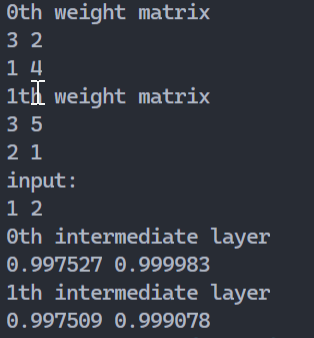
\includegraphics[width=0.5\textwidth]{./image/annfp}
    \caption{The results}
\end{figure}

\end{homeworkProblem}

\end{document}
